\documentclass[12pt]{article}
\usepackage[utf8]{inputenc}
\usepackage[margin=0.7in]{geometry}
\usepackage{titlesec}
\usepackage{graphicx}
\usepackage[english]{babel}
\usepackage{fancyhdr}
\usepackage{blindtext}
\usepackage{textcomp}
\usepackage{pgfplots}
\titlespacing\section{0pt}{14pt plus 4pt minus 2pt}{0pt plus 2pt minus 2pt}
\newlength\tindent
\setlength{\tindent}{\parindent}
\setlength{\parindent}{0pt}
\renewcommand{\indent}{\hspace*{\tindent}}
\pagestyle{fancy}
\fancyhf{}
\rhead{Sam Robbins 13SE}
\lhead{A Level Physics - Turning Points}

\usepackage{tikz}
\usetikzlibrary{scopes}


\usepackage{mathtools}

\newtagform{brackets}{[}{]}
\usetagform{brackets}

\begin{document}
\begin{center}
\underline{\huge Electrons}
\end{center}
\section{Discharge tube}
\begin{itemize}
\item As p.d. increased from 0V, initially no glow
\item p.d. increased further - suddenly glows can be seen and p.d. drops as the gas now conducts
\item Increasing p.d. further causes gas to glow brighter
\end{itemize}
When several kV is applied a narrow band "glow" causes gas to glow brighter
\subsection{Explanation of how it works}
\begin{itemize}
\item The high p.d. is sufficient to ionise the gas
\item The positive ions accelerate towards the cathode
\item The ions will hit the metal cathode with sufficient energy to release free electrons from the surface
\item The free electrons from the metal (low energy) can recombine with the gas ions-emitting photons and will be a continuous spectrum
\item The free electrons accelerate towards the anode. These free electrons will \textbf{inelastically} collide with gas atoms (and ions) causing bound electrons to be excited, then de-excited. This will produce a discrete spectrum which is seen in the positive column.
\end{itemize}
\section{Thermionic emission}
When a metal is heated the free electrons can gain enough energy to be released from the surface. This is called thermionic emission (similar to the photoelectric effect).\\
\\
In the presence of an electric field the thermionic electrons can be accelerated to form a narrow beam.\\
\\
When accelerated through a p.d. of \textbf{V} volts the electron gains \textbf{eV} in energy in the form of kinetic energy.
\newpage
\section{Determining the specific charge of an electron}
\subsection{Method 1}
1. Thermionic electrons are accelerated through a p.d. $V_a$ and gain kinetic energy:\\
$$eV_a=\frac{1}{2}mv^2 \quad \frac{e}{m}=\frac{\frac{1}{2}v^2}{v_a}$$
2. Electrons pass through an electric field (Field strength, E) and are deflected.\\
\\
3. A magnetic field (field strength, B) is applied at right angles to the E field until electron motion is again horizontal.
$$\textrm{At this point magnetic force=Electric force}$$
$$Bev=eE \quad v=\frac{E}{B}$$
$$\frac{e}{m}=\frac{1}{2v_a}\Bigg(\frac{E}{B}\Bigg)^2$$
\subsection{Method 2}
\includegraphics[width=10cm]{circluar_path.jpg}\\
Thermionic electrons are accelerated through a p.d. $V_a$\\
A magnetic field is applied perpendicular to the motion, causing the electrons to feel a force.\\
\\
$$\textrm{Magnetic force   F=Bev}$$
$$\textrm{This is the centripetal force} \frac{mv^2}{R}$$
$$\frac{e}{m}=\frac{v}{BR} \quad \quad v=\frac{e}{m}BR$$
$$\textrm{From accelerating p.d.}\quad eV_a=\frac{1}{2}mv^2$$
$$\frac{e}{m}=\frac{2V_a}{(BR)^2}$$
\newpage
\section{Milikan's experiment}
\begin{figure}[h]
    \centering
    \begin{minipage}{0.45\textwidth}
        \centering
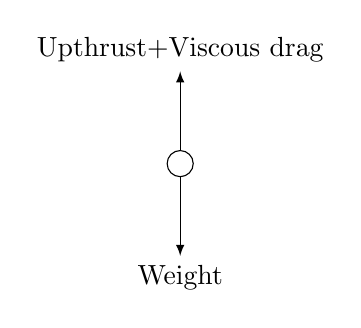
\begin{tikzpicture}[
    force/.style={>=latex,draw=black,fill=black},
    m/.style={circle,draw=black,fill=white,radius=0.3cm,thin},
]
    \node[m] (m) {};
    {[force,->]
        \draw (m.north) -- ++(0,1) node[above] {Upthrust+Viscous drag};
        \draw (m.south) -- ++(0,-1) node[below] {Weight};
    }
\end{tikzpicture}
        \caption{No electric field}
    \end{minipage}\hfill
    \begin{minipage}{0.45\textwidth}
        \centering
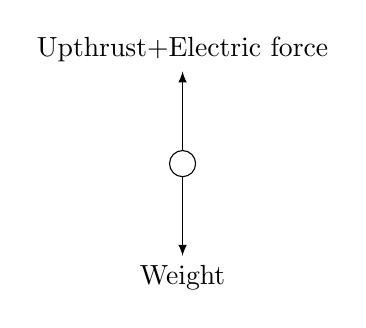
\begin{tikzpicture}[
    force/.style={>=latex,draw=black,fill=black},
    m/.style={circle,draw=black,fill=white,radius=0.3cm,thin},
]
    \node[m] (m) {};
    {[force,->]
        \draw (m.north) -- ++(0,1) node[above] {Upthrust+Electric force};
        \draw (m.south) -- ++(0,-1) node[below] {Weight};
    }
\end{tikzpicture}    
        \caption{Electric field}
    \end{minipage}
\end{figure}
\subsection{With electric field}
$$\textrm{Electric field}=\frac{QV}{d}$$
$$\textrm{Weight}=mg$$
$$\frac{QV}{d}=mg$$
\subsection{Without electric field}
$$F_D=6\pi r\eta v$$
$$\textrm{Weight}=mg$$
\begin{center}
Mass=Density$\times$Volume
$$\textrm{Mass}=\frac{4}{3}\pi r^3\rho$$
$$6\pi r\eta v=\frac{4}{3}\pi r^3\rho g$$
$$r^2=\frac{9\eta v}{2\rho g}$$
\end{center}
\subsection{Significance of results}
These results were significant because it introduced the idea of quantisation of charge


\end{document}